\chapter{10 Questions with a Real Estate Millionaire: Scale, Brokerage, and Contract Control}

This interview unfolds like a short lecture in commercial scale. We are first shown, almost before we know where we are, a profession in which a single check can be \(200{,}000\), and then a first commission earned while the speaker is still delivering pizza and mopping floors. From there the discussion widens into the layered acquisition of real-estate knowledge, narrows again into the institutional passage from agent to broker, turns outward toward partnership and leadership, and finally lands on a worked example in wholesaling. The mathematics here is not blackboard mathematics. It is the arithmetic of thresholds, splits, contract control, and gain.

\section{Cold Open: Money Becomes Visible}

The interview does not begin with biography. It begins with scale. Matt Teifke recalls meeting a local broker and seeing a \(200{,}000\) check come across the desk. That scene matters because it changes the unit by which the profession is measured. Wealth is not yet a theory; it is an object in the room.

The story then immediately drops us back to ordinary wage life. Teifke is still working at Papa John's, still mopping floors, when his first real-estate call comes in. He takes the call, closes the deal, and remembers receiving a commission on the order of \(6{,}000\) to \(7{,}000\). These three scales belong together:
\begin{align}
B_{\mathrm{observed}} &= 200{,}000, &
W_{\mathrm{ordinary}} &\approx 600, &
F_{\mathrm{first}} &\in [6{,}000,7{,}000].
\end{align}

The corresponding comparisons are elementary, but they explain the emotional force of the opening:
\begin{equation}
\frac{F_{\mathrm{first}}}{W_{\mathrm{ordinary}}} \in [10,11.67],
\qquad
\frac{B_{\mathrm{observed}}}{W_{\mathrm{ordinary}}} \approx 333.
\end{equation}

So the cold open is not merely motivational rhetoric. It is a lesson in scale compression. One event in the new domain outweighs many cycles in the old one.

\begin{remark}
The transcript reports both \(6{,}000\) and \(7{,}000\) for the first commission. It is better to preserve the uncertainty than to pretend the spoken record is exact.
\end{remark}

\section{Building the Stack}

Only after this jolt of scale does the interview formally identify the guest and the project: Teifke Real Estate and the stated ambition to build the most entrepreneurial brokerage on the planet. From there the speaker does not present a miracle. He presents a stack.

The stack is worth keeping in order:
\begin{itemize}
\item family influence, especially through a mother who showed what real estate could make possible,
\item licensing at age \(17\),
\item a small brokerage where he was first in and last out,
\item commercial brokerage experience,
\item a master's degree in real estate with a financial emphasis,
\item appraisal training,
\item apartment work,
\item third-party property management up to roughly \(700\) doors,
\item the sale of that management company,
\item a later entrepreneurial brokerage built with Alex Kaufman.
\end{itemize}

The point of this sequence is structural. Each layer gives contact with a different piece of the real-estate machine. When the speaker later discusses broker licensing, split structures, or wholesaling, he is not speaking from one narrow perch. He has moved through several adjacent institutions.

\subsection{College as Network, Not Credential}

At this point the interviewer poses the first conceptual test: did college matter, and is it necessary?

Teifke's answer is subtle. Necessary? No. Useful? Yes, if one uses it properly. He describes teaching a college class and tells students, in effect, that ten people in a room who are all interested in business already possess a latent asset. The asset is not merely the credential at the end. The asset is the coordination possibility in the middle.

This is a genuine pivot in the lecture. We move from biography to method. A school, like a brokerage, has value only if one enters it actively. In this sense the interview is already teaching a general rule: institutions are not enough, but institutions can be exploited.

\section{Entering the Market}

The interviewer now circles back. This is an important narrative move. We have the broad arc, but we do not yet have the decisive scene in which a beginner actually discovers how the market behaves.

Teifke describes showing up to brokerage interviews in a suit and tie, hoping he might be given a job. The reversal is immediate. He later realizes that almost every brokerage wants new agents. The novice thinks he is entering a gatekeeping market. The market is in fact recruiting him.

\subsection{Question \& Answer}

\paragraph{Question.} How does a young agent actually break in?

\paragraph{Answer.} The answer has two parts, and the lecture keeps them in the right order. First, one has to learn that the market is not organized as the beginner imagines it. The brokerages are not merely judges; they are also seekers of new agents. Second, one has to experience scale personally. The \(200{,}000\) check proves that the profession can produce large gains. The first commission proves that the speaker himself can participate in that world.

That is why the Papa John's scene matters so much. It is not just an origin anecdote. It is the moment at which an ordinary wage horizon breaks open. Once \(F_{\mathrm{first}}\) arrives, the profession stops looking hypothetical. The speaker says plainly that he was hooked.

\section{From Agent to Broker}

Once the first deal has done its work, the interview moves from entry to structure. The new question is not how one gets in, but how one moves up.

The first institutional fact is sharp: an agent cannot operate in the business without a broker. The broker is the legal and operational umbrella. The second fact is that the threshold changed during the speaker's own progression. What had been a two-year requirement became a four-year requirement just as he was approaching it. The threshold, in other words, receded.

We may summarize the reported licensing conditions as
\begin{align}
y_{\mathrm{broker,old}} &\ge 2,
&
y_{\mathrm{broker,now}} &\ge 4,
&
N_{\mathrm{pts}} &\gtrsim 900.
\end{align}

The last quantity is stated conversationally, so it should be read as approximate. Even so, the structure is clear. Broker status is a threshold problem involving time, transactions, points, and coursework. Teifke also notes that his college and master's work satisfied the classroom-credit portion of the requirement.

\subsection{Question \& Answer}

\paragraph{Question.} What changes when one moves from agent to broker?

\paragraph{Answer.} Two things change at once. First, the person now stands on the hook legally and operationally: responsible, supervising, training, and supporting. Second, the economics of the brokerage become visible as a split system.

Let \(C\) denote gross commission on a deal. The interview gives the current and earlier splits as
\begin{align}
C_{\mathrm{agent}} &= 0.9C, &
C_{\mathrm{firm}} &= 0.1C, \\
C_{\mathrm{agent,old}} &= 0.5C, &
C_{\mathrm{firm,old}} &= 0.5C.
\end{align}

The agent-side improvement is therefore
\begin{align}
C_{\mathrm{agent}} - C_{\mathrm{agent,old}}
&= 0.9C - 0.5C \\
&= 0.4C.
\end{align}

If we take a simple example with \(C=10{,}000\), then
\begin{equation}
C_{\mathrm{agent}} = 9{,}000,
\qquad
C_{\mathrm{agent,old}} = 5{,}000,
\qquad
C_{\mathrm{agent}} - C_{\mathrm{agent,old}} = 4{,}000.
\end{equation}

\begin{table}[h]
\centering
\caption{Commission split structures described in the interview}
\begin{tabular}{|c|c|c|}
\hline
Structure & Agent share & Firm share \\
\hline
Current brokerage & \(90\%\) & \(10\%\) \\
First brokerage & \(50\%\) & \(50\%\) \\
\hline
\end{tabular}
\end{table}

This is the place where the lecture turns from the arithmetic of gain to the arithmetic of responsibility. The broker gets a piece of the deal, but the broker also becomes the person who must answer for the agents.

\begin{remark}
The reported \(900\)-point threshold is best treated as a speaker-reported figure rather than a verified regulatory constant.
\end{remark}

\section{Leadership, Pressure, and Partnership}

Once brokerage structure is on the table, the interview asks what it feels like to bear it. Teifke's answer is not glamorous. The hard part of owning a brokerage is not merely growth. It is leadership under visible strain: deals falling apart, complaints arriving, lawsuits appearing, and the necessity of showing up anyway.

That prepares the next movement into partnership. The speaker gives a rough base-rate claim that perhaps one in twenty partnerships works. He then slows down and explains why this one did. The tension is not hidden. Alex Kaufman is not introduced as an obvious safe partner. He is introduced through past addiction, jail, and the speaker's own reluctance to associate closely. Trust is therefore not assumed; it is built.

The test is behavioral. Give him ten doors and he knocks one hundred. Give him a list of calls and he makes many more than requested. Over time they own four or five properties together. Over time the speaker becomes persuaded that the sobriety is real, the discipline is real, and the direction of the life is real.

The final resolution of the section is functional. The partnership works because it divides labor rather than duplicating it.
\begin{table}[h]
\centering
\caption{Functional division inside the partnership}
\begin{tabular}{|c|c|}
\hline
Alex & Matt Teifke \\
\hline
operations & networking \\
profitability & relationship building \\
hiring and firing & new ideas \\
money discipline & outward growth \\
\hline
\end{tabular}
\end{table}

Late in the segment the speaker gives the entrepreneurial shorthand: Alex is the implementer, Teifke the visionary. The notes should keep the phrase, but its content is practical. It names a division of function, not a mood board.

\section{Biggest Deal: Contract Control and Wholesaling}

The interviewer next asks about best and worst financial decisions and also about the biggest deal. Teifke answers the biggest-deal question first. That order is worth preserving, because the lecture wants to put a concrete commercial mechanism on the table before it returns to judgment more broadly.

The deal concerns roughly nine and a half acres in Round Rock. The speaker and his partners place the property under contract, post earnest and option money, and then search for builders and developers who might pay more. The core idea is that control of the contract is itself economically valuable.

\begin{definition}
In the usage of this interview, wholesaling is the monetization of contractual control. One puts a property under contract, commits the money needed to control that paper, and then finds a buyer willing to pay enough to make the transfer profitable.
\end{definition}

\subsection{Question \& Answer}

\paragraph{Question.} What, exactly, is being sold in wholesaling?

\paragraph{Answer.} The interview's answer is compact but precise. One is not simply buying land and then passively owning it. One is controlling the deal through the contract. The property matters, but the operative instrument is the paper that gives the right to close, assign, or transfer.

The numerical data reported in the interview are these:
\begin{align}
P_0 &= 2.0\times 10^6,
&
P_1 &= 2.7\times 10^6,
&
\Delta P &= P_1-P_0 = 0.7\times 10^6, \\
K_0 &= E+O \approx 20{,}000,
&
F_{\mathrm{wholesale}} &\in [700{,}000,780{,}000],
&
C_{\mathrm{broker}} &= 0.03P.
\end{align}

Here \(P_0\) is the contract price, \(P_1\) is the later buyer's offer, \(K_0\) is the earnest-plus-option money used to control the contract, \(F_{\mathrm{wholesale}}\) is the stated wholesale fee, and \(C_{\mathrm{broker}}\) is the separate commission term the speaker says also went to their side.

Because the interview compresses several financial streams into one story, it is best to separate them symbolically:
\begin{equation}
G = F_{\mathrm{wholesale}} + C_{\mathrm{broker}},
\qquad
N_{\mathrm{partner}} \approx \frac{G-T}{3},
\end{equation}
where \(G\) is gross proceeds before partner split and \(T\) stands for taxes and any other reductions before net.

A schematic picture of the mechanism is useful.

\begin{figure}[h]
\centering
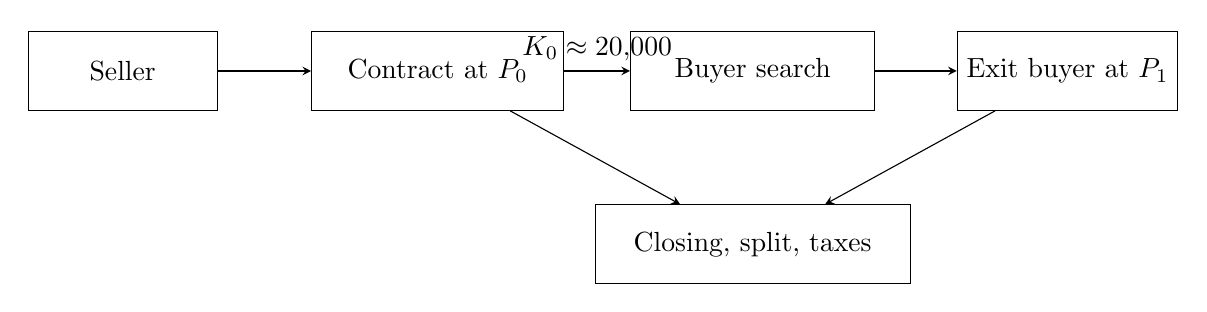
\begin{tikzpicture}[>=stealth]
\node[draw, rectangle, minimum width=2.4cm, minimum height=1cm] (seller) at (0,0) {Seller};
\node[draw, rectangle, minimum width=3.2cm, minimum height=1cm] (contract) at (4,0) {Contract at \(P_0\)};
\node[draw, rectangle, minimum width=3.1cm, minimum height=1cm] (search) at (8,0) {Buyer search};
\node[draw, rectangle, minimum width=2.8cm, minimum height=1cm] (buyer) at (12,0) {Exit buyer at \(P_1\)};
\node[draw, rectangle, minimum width=4cm, minimum height=1cm] (close) at (8,-2.2) {Closing, split, taxes};

\draw[->] (seller) -- (contract);
\draw[->] (contract) -- node[above] {\(K_0 \approx 20{,}000\)} (search);
\draw[->] (search) -- (buyer);
\draw[->] (buyer) -- (close);
\draw[->] (contract) -- (close);
\end{tikzpicture}
\caption{Editorial reconstruction from the transcript: wholesaling as contract control, buyer search, and closing.}
\end{figure}

We can now write the example in the order the lecture itself suggests.
\begin{enumerate}
\item Secure the property under contract at \(P_0=2.0\times 10^6\).
\item Put up approximately \(K_0=20{,}000\) in earnest and option money.
\item Use the contract to control the opportunity while searching for builders, developers, and other buyers.
\item Receive an offer at \(P_1=2.7\times 10^6\).
\item Observe that the raw spread is
\[
\Delta P = P_1-P_0 = 0.7\times 10^6.
\]
\item Keep the spread separate from the reported wholesale fee \(F_{\mathrm{wholesale}}\), because the transcript states the latter directly and somewhat unstably.
\item Keep the commission term \(C_{\mathrm{broker}}\) separate as well.
\end{enumerate}

For a single illustrative calculation, let us temporarily take the commission base to be the contract price \(P_0\). Then
\begin{equation}
C_{\mathrm{broker}} \approx 0.03\times 2.0\times 10^6 = 60{,}000.
\end{equation}

Under that particular assumption,
\begin{equation}
G \in [760{,}000,840{,}000].
\end{equation}

A three-way pre-tax split would then be
\begin{equation}
\frac{G}{3} \in [253{,}333,280{,}000].
\end{equation}

The speaker, however, insists on a more sober reading than the headline suggests. One pays large taxes, and the net is therefore materially smaller than the visible gross. That caution belongs to the mathematics, not merely to the rhetoric.

\begin{remark}
Three uncertainties should remain visible. First, the transcript gives both \(700{,}000\) and \(780{,}000\) for the wholesale fee. Second, the base price in \(C_{\mathrm{broker}}=0.03P\) is not explicitly fixed. Third, the spread \(\Delta P\) should not be identified mechanically with the wholesale fee. The interview supports these as related quantities, not as identical ones.
\end{remark}

\section{Bad Bets, Strange Days, and the Long Horizon}

After the biggest deal, the interviewer circles back to the broader question of best and worst financial decisions. This return is important. A great deal does not settle the question of judgment.

The worst decision, as Teifke tells it, is cannabis stock. The crucial feature is daily volatility. The investment is not described merely as having gone down once. It is described as a position that can move violently from day to day:
\begin{equation}
|\Delta V_{\mathrm{cannabis,day}}| \in [60{,}000,100{,}000].
\end{equation}

He also gives two speaker-reported corporate metrics:
\begin{equation}
R_Q \approx 67\times 10^6,
\qquad
V_{\mathrm{equity}} \approx 40\times 10^6.
\end{equation}

These numbers are not used in the interview to prove a valuation theorem. They function differently. They show the speaker trying to reconcile deep drawdown with a continued belief that the underlying business is undervalued.

The best decision, by contrast, is not a trade or a parcel. It is the decision to partner with Alex. That answer retrospectively confirms the structure of the whole chapter: people, roles, and institutions precede windfalls.

The ``craziest story'' segment then reminds us that the business itself remains stubbornly physical and disorderly. A pregnant wife is chased by a tenant with a stick and a dog; an RV-park conversation becomes a negotiation over a beer. The lecture refuses to let wealth-building become an abstract spreadsheet detached from field conditions.

The final question is about the next ten years and what keeps the speaker going. Here the interview leaves arithmetic and returns to orientation. The answer is not constant emotional intensity. It is clarity of direction. He says, in effect, that one must know where one is trying to go, and that the daily proof of meaning comes from agents who say their lives have changed.

We may summarize the long-horizon scale markers mentioned late in the interview by
\begin{equation}
N_{\mathrm{properties}} \approx 130,
\qquad
|\Delta V_{\mathrm{cannabis,day}}| \in [60{,}000,100{,}000].
\end{equation}

Again the point is not to build a full balance-sheet model. It is to register how large operating scale and large uncertainty coexist.

\section{Summary}

The interview begins with a check, not a theory. That is its first lesson. Scale has to be seen before it can be believed. From there the discussion builds step by step: a layered formation in real estate, a reframing of college as a coordination environment, a rewind to the actual mechanics of getting started, the threshold problem of becoming a broker, the burdens of leadership, the functional logic of partnership, and finally a wholesaling example in which contractual control becomes monetizable.

The strongest mathematical content of the chapter lies in simple but consequential structures: ratios of pay scales, threshold inequalities for broker licensing, split formulas for commissions, and a worked arithmetic example for wholesaling. None of this is advanced mathematics. But it is disciplined commercial mathematics. It shows us how an interview about wealth can become, if we read it carefully, a lecture about units, thresholds, control, and responsibility.

The last note should be kept in view. The lecture does not end by celebrating the biggest fee. It ends by returning to direction. Clear goals, repeated effort, and the ability to change other people's lives form the long-run frame in which all the earlier arithmetic is meant to sit.